\section{هدف تمرین}
در این سؤال، یک صف سنکرون (\lr{Synchronous FIFO}) با استفاده از یک میان‌گیر چرخشی (\lr{Circular Buffer}) و آرایه‌ی دو بعدی از ثبات‌ها طراحی و پیاده‌سازی شده است. این مدار هر دو عملیات خواندن و نوشتن را در یک چرخه‌ی ساعت انجام داده و وضعیت پر یا خالی بودن صف را نیز به کمک یک شمارنده‌ی داخلی نگه‌داری می‌کند.


\section{توضیح معماری}

صف سنکرون از بخش‌های اصلی زیر تشکیل شده است:

\begin{itemize}
    \item \textbf{حافظه چرخشی (\code{fifo\_mem}):} یک آرایه دو بعدی از ثبات‌ها به ابعاد \code{FIFO\_DEPTH} $\times$ \code{DATA\_WIDTH}.
    \item \textbf{اشاره‌گرها (\code{wr\_ptr} و \code{rd\_ptr}):} ثبات‌های \code{ADDR\_WIDTH} بیتی که آدرس خانه بعدی برای نوشتن و خواندن را مشخص می‌کنند و با هر عملیات یک واحد افزایش می‌یابند (با سرریز طبیعی آدرس‌ها دور می‌زنند).
    \item \textbf{شمارنده عناصر (\code{count}):} ثبات \code{ADDR\_WIDTH + 1} بیتی برای ذخیره‌ی تعداد عناصر موجود در صف (از $0$ تا \code{FIFO\_DEPTH}).
\end{itemize}

منطق تشخیص وضعیت پر و خالی بودن مدار به صورت ترکیبی و مستقیم از روی شمارنده محاسبه می‌شود:
\begin{latin}
    \begin{lstlisting}[language=Verilog]
assign empty = (count == 0);
assign full  = (count == FIFO_DEPTH);
\end{lstlisting}
\end{latin}

در حالت درخواست همزمان خواندن و نوشتن (\code{wr\_en=1} و \code{rd\_en=1}):
\begin{itemize}
    \item اگر صف نه خالی باشد و نه پر، هر دو عملیات انجام شده و \code{count} تغییر نمی‌کند.
    \item اگر صف خالی باشد (\code{empty=1})، فقط نوشتن معتبر است و \code{count} یک واحد افزایش می‌یابد.
    \item اگر صف پر باشد (\code{full=1})، فقط خواندن معتبر است و \code{count} یک واحد کاهش می‌یابد.
\end{itemize}


\section{توضیح کد}

\subsection{ماژول \code{sync\_fifo}}
این ماژول عملیات بازنشانی سنکرون، به‌روزرسانی اشاره‌گرها، نوشتن در حافظه، خواندن روی خروجی \code{dout} و مدیریت شمارنده \code{count} را در لبه بالارونده کلک انجام می‌دهد. کد اصلی مدار به این صورت می‌باشد:

\vspace{0.4cm}
\begin{latin}
    \begin{lstlisting}[language=Verilog]
always @(posedge clk) begin
    if (rst) begin
        wr_ptr <= {ADDR_WIDTH{1'b0}};
        rd_ptr <= {ADDR_WIDTH{1'b0}};
        count  <= {(ADDR_WIDTH+1){1'b0}};
        dout   <= {DATA_WIDTH{1'b0}};
    end else begin
        // Write Operation
        if ((wr_en && !full) || (wr_en && rd_en && empty)) begin
            fifo_mem[wr_ptr] <= din;
            wr_ptr <= wr_ptr + 1'b1;
        end

        // Read Operation
        if ((rd_en && !empty) || (wr_en && rd_en && full)) begin
            dout <= fifo_mem[rd_ptr];
            rd_ptr <= rd_ptr + 1'b1;
        end

        // Counter Logic
        case ({wr_en, rd_en})
            2'b10: if (!full)  count <= count + 1'b1; // Write only
            2 me01: if (!empty) count <= count - 1'b1; // Read only
            2'b11: begin                              // Simultaneous R/W
                if (empty)      count <= count + 1'b1;
                else if (full) count <= count - 1'b1;
            end
            default: ;
        endcase
    end
end
\end{lstlisting}
\end{latin}

\subsection{تست‌بنچ}

\textbf{تسک \code{check\_step}:}
این تسک پس از لبه‌ی فعال ساعت با یک واحد تأخیر (\code{\#1}) مقادیر سیگنال‌های ورودی (\code{rst}، \code{din}، \code{wr\_en} و \code{rd\_en})، خروجی‌های \lr{DUT} و مقادیر مورد انتظار را در ترمینال چاپ کرده و در صورت عدم تطابق، متغیر \code{tc\_failed} را یک می‌کند:

\vspace{0.4cm}
\begin{latin}
    \begin{lstlisting}[language=Verilog]
task check_step;
    input [DATA_WIDTH-1:0] exp_dout;
    input exp_full, exp_empty;
    begin
        #1; // Delay for non-blocking assignments
        $display("  [Cycle %02d] IN: rst=%b din=0x%02h wr=%b rd=%b | DUT: dout=0x%02h full=%b empty=%b | EXP: dout=0x%02h full=%b empty=%b",
                 cycle_num, rst, din, wr_en, rd_en, dout, full, empty, exp_dout, exp_full, exp_empty);

        if (dout !== exp_dout || full !== exp_full || empty !== exp_empty) begin
            $display("       [ERROR] Mismatch at cycle %02d!", cycle_num);
            tc_failed = 1;
        end
    end
endtask
\end{lstlisting}
\end{latin}

\textbf{تسک‌های کمک‌کننده:}
تست‌بنچ از ۴ تسک اصلی برای اعمال ورودی‌ها روی لبه‌ی پایین کلک (\code{negedge clk}) و ارزیابی خروجی در لبه‌ی بالایی بعد استفاده می‌کند:
\begin{itemize}
    \item \code{apply\_reset}: سیگنال \code{rst=1} را اعمال کرده و پس از یک سیکل، خالی بودن صف را ارزیابی می‌کند.
    \item \code{do\_write}: مقدار ورودی \code{din} را قرار داده، \code{wr\_en=1} می‌کند و صحّت خروجی‌ها را بررسی می‌نماید.
    \item \code{do\_read}: سیگنال \code{rd\_en=1} را فعال کرده و داده‌ی خوانده‌شده روی \code{dout} را ارزیابی می‌کند.
    \item \code{do\_both}: هر دو سیگنال \code{wr\_en=1} و \code{rd\_en=1} را همزمان فعال کرده و رفتار مدار در شرایط مختلف را می‌سنجد.
\end{itemize}

\textbf{تست‌کیس‌ها:}

تست‌های اصلی به ترتیب زیر اجرا می‌شوند:

\vspace{0.4cm}
\begin{latin}
    \begin{lstlisting}[language=Verilog]
// Test 1: Synchronous Reset
tc_failed = 0;
apply_reset();
finish_test_case("Synchronous Reset");
\end{lstlisting}
\end{latin}

\vspace{-0.2cm}
با اعمال \code{rst} در لبه‌ی فعال ساعت، تمامی اشاره‌گرها و شمارنده‌ی داخلی صفر شده و بررسی می‌شود که \code{empty=1} و \code{full=0} باشد.

\vspace{0.8cm}
\begin{latin}
    \begin{lstlisting}[language=Verilog]
// Test 2: Sequential Writes and Reads (FIFO ordering)
tc_failed = 0;
apply_reset();
do_write(8'hA1, 8'h00, 1'b0, 1'b0);
do_write(8'hA2, 8'h00, 1'b0, 1'b0);
do_write(8'hA3, 8'h00, 1'b0, 1 me0);
do_write(8'hA4, 8'h00, 1'b0, 1'b0);
do_read(8'hA1, 1'b0, 1'b0);
do_read(8'hA2, 1'b0, 1'b0);
do_read(8'hA3, 1'b0, 1'b0);
do_read(8'hA4, 1'b0, 1'b1);
finish_test_case("Sequential Write / Read / FIFO Order");
\end{lstlisting}
\end{latin}

\vspace{-0.2cm}
۴ داده‌ی متوالی در صف نوشته شده و سپس به ترتیب خوانده می‌شوند تا حفظ ترتیب ورود و خروج (\lr{FIFO order}) و فعال شدن \code{empty=1} پس از خواندن آخرین داده تأیید شود.

\vspace{0.8cm}
\begin{latin}
    \begin{lstlisting}[language=Verilog]
// Test 3: Fill Completely + Write-to-Full Ignored
tc_failed = 0;
apply_reset();
for (i = 0; i < FIFO_DEPTH; i = i + 1)
    do_write(8'h10 + i, 8'h00, (i == FIFO_DEPTH - 1), 1'b0);
do_write(8'hFF, 8'h00, 1'b1, 1'b0); // Sentinel write to full FIFO
do_read(8'h10, 1'b0, 1'b0);         // Verify head data remains 0x10
finish_test_case("Fill Completely + Write-to-Full Ignored");
\end{lstlisting}
\end{latin}

\vspace{-0.2cm}
صف به میزان \code{FIFO\_DEPTH} خانه پر شده تا \code{full=1} گردد. سپس یک داده‌ی اضافی (\code{0xFF}) روی صف پر نوشته می‌شود؛ در مرحله‌ی بعد با خواندن اولین عنصر بررسی می‌شود که داده‌ی اضافی نادیده گرفته شده و داده‌ی اصلی سر صف تغییر نکرده باشد.

\vspace{0.8cm}
\begin{latin}
    \begin{lstlisting}[language=Verilog]
// Test 4: Drain Completely + Read-from-Empty Ignored
tc_failed = 0;
apply_reset();
for (i = 0; i < FIFO_DEPTH; i = i + 1)
    do_write(8'h20 + i, 8'h00, (i == FIFO_DEPTH - 1), 1'b0);
for (i = 0; i < FIFO_DEPTH; i = i + 1)
    do_read(8'h20 + i, 1'b0, (i == FIFO_DEPTH - 1));
do_read(8'h20 + FIFO_DEPTH - 1, 1'b0, 1'b1); // Spurious read from empty
finish_test_case("Drain Completely + Read-from-Empty Ignored");
\end{lstlisting}
\end{latin}

\vspace{-0.2cm}
صف ابتدا کاملاً پر شده و سپس تمام داده‌های آن خوانده می‌شوند تا \code{empty=1} گردد. درخواست خواندن مجدد روی صف خالی اعمال شده و بررسی می‌شود که عملیات نادیده گرفته شده و \code{empty=1} باقی بماند.

\vspace{0.8cm}
\begin{latin}
    \begin{lstlisting}[language=Verilog]
// Test 5: Simultaneous RW: Normal State
tc_failed = 0;
apply_reset();
for (i = 0; i < 8; i = i + 1)
    do_write(8'h30 + i, 8'h00, 1'b0, 1'b0);
do_both(8'h40, 8'h30, 1'b0, 1'b0);
do_both(8'h41, 8'h31, 1'b0, 1'b0);
do_both(8'h42, 8'h32, 1'b0, 1'b0);
do_both(8'h43, 8'h33, 1'b0, 1'b0);
finish_test_case("Simultaneous RW: Normal State");
\end{lstlisting}
\end{latin}

\vspace{-0.2cm}
در حالت نیمه‌پر، عملیات خواندن و نوشتن همزمان (\code{do\_both}) اجرا می‌شود. صحت خروجی داده‌ی خوانده‌شده بررسی شده و تأیید می‌گردد که تعداد عناصر موجود در صف (\code{count}) تغییر نکرده است.

\vspace{0.8cm}
\begin{latin}
    \begin{lstlisting}[language=Verilog]
// Test 6: Simultaneous RW: FIFO Empty
tc_failed = 0;
apply_reset();
do_both(8'hAB, 8'h00, 1'b0, 1'b0);  // Simultaneous RW on empty FIFO
do_read(8'hAB, 1'b0, 1'b1);         // Read back newly written byte
finish_test_case("Simultaneous RW: FIFO Empty");
\end{lstlisting}
\end{latin}

\vspace{-0.2cm}
روی صف خالی درخواست همزمان خواندن و نوشتن داده می‌شود. طبق منطق مدار، فقط عملیات نوشتن باید معتبر باشد؛ بلافاصله با یک خواندن مجدد، دریافت داده‌ی جدید (\code{0xAB}) ارزیابی می‌گردد.

\vspace{0.8cm}
\begin{latin}
    \begin{lstlisting}[language=Verilog]
// Test 7: Simultaneous RW: FIFO Full
tc_failed = 0;
apply_reset();
for (i = 0; i < FIFO_DEPTH; i = i + 1)
    do_write(8'h50 + i, 8'h00, (i == FIFO_DEPTH - 1), 1'b0);
do_both(8'hFF, 8'h50, 1'b0, 1'b0);  // Simultaneous RW on full FIFO
do_read(8'h51, 1'b0, 1'b0);         // Confirm next item intact (0xFF was ignored)
finish_test_case("Simultaneous RW: FIFO Full");
\end{lstlisting}
\end{latin}

\vspace{-0.2cm}
روی صف پر درخواست همزمان خواندن و نوشتن اعمال می‌شود. در این حالت فقط خواندن معتبر است؛ با بررسی داده‌ی خوانده‌شده بعدی (\code{0x51}) تأیید می‌شود که داده‌ی جدید (\code{0xFF}) نوشتن نشده است.

\pagebreak

\section{اجرای کد}
نتیجه‌ی اجرای کد به این صورت می‌باشد:

\begin{figure}[H]
    \centering
    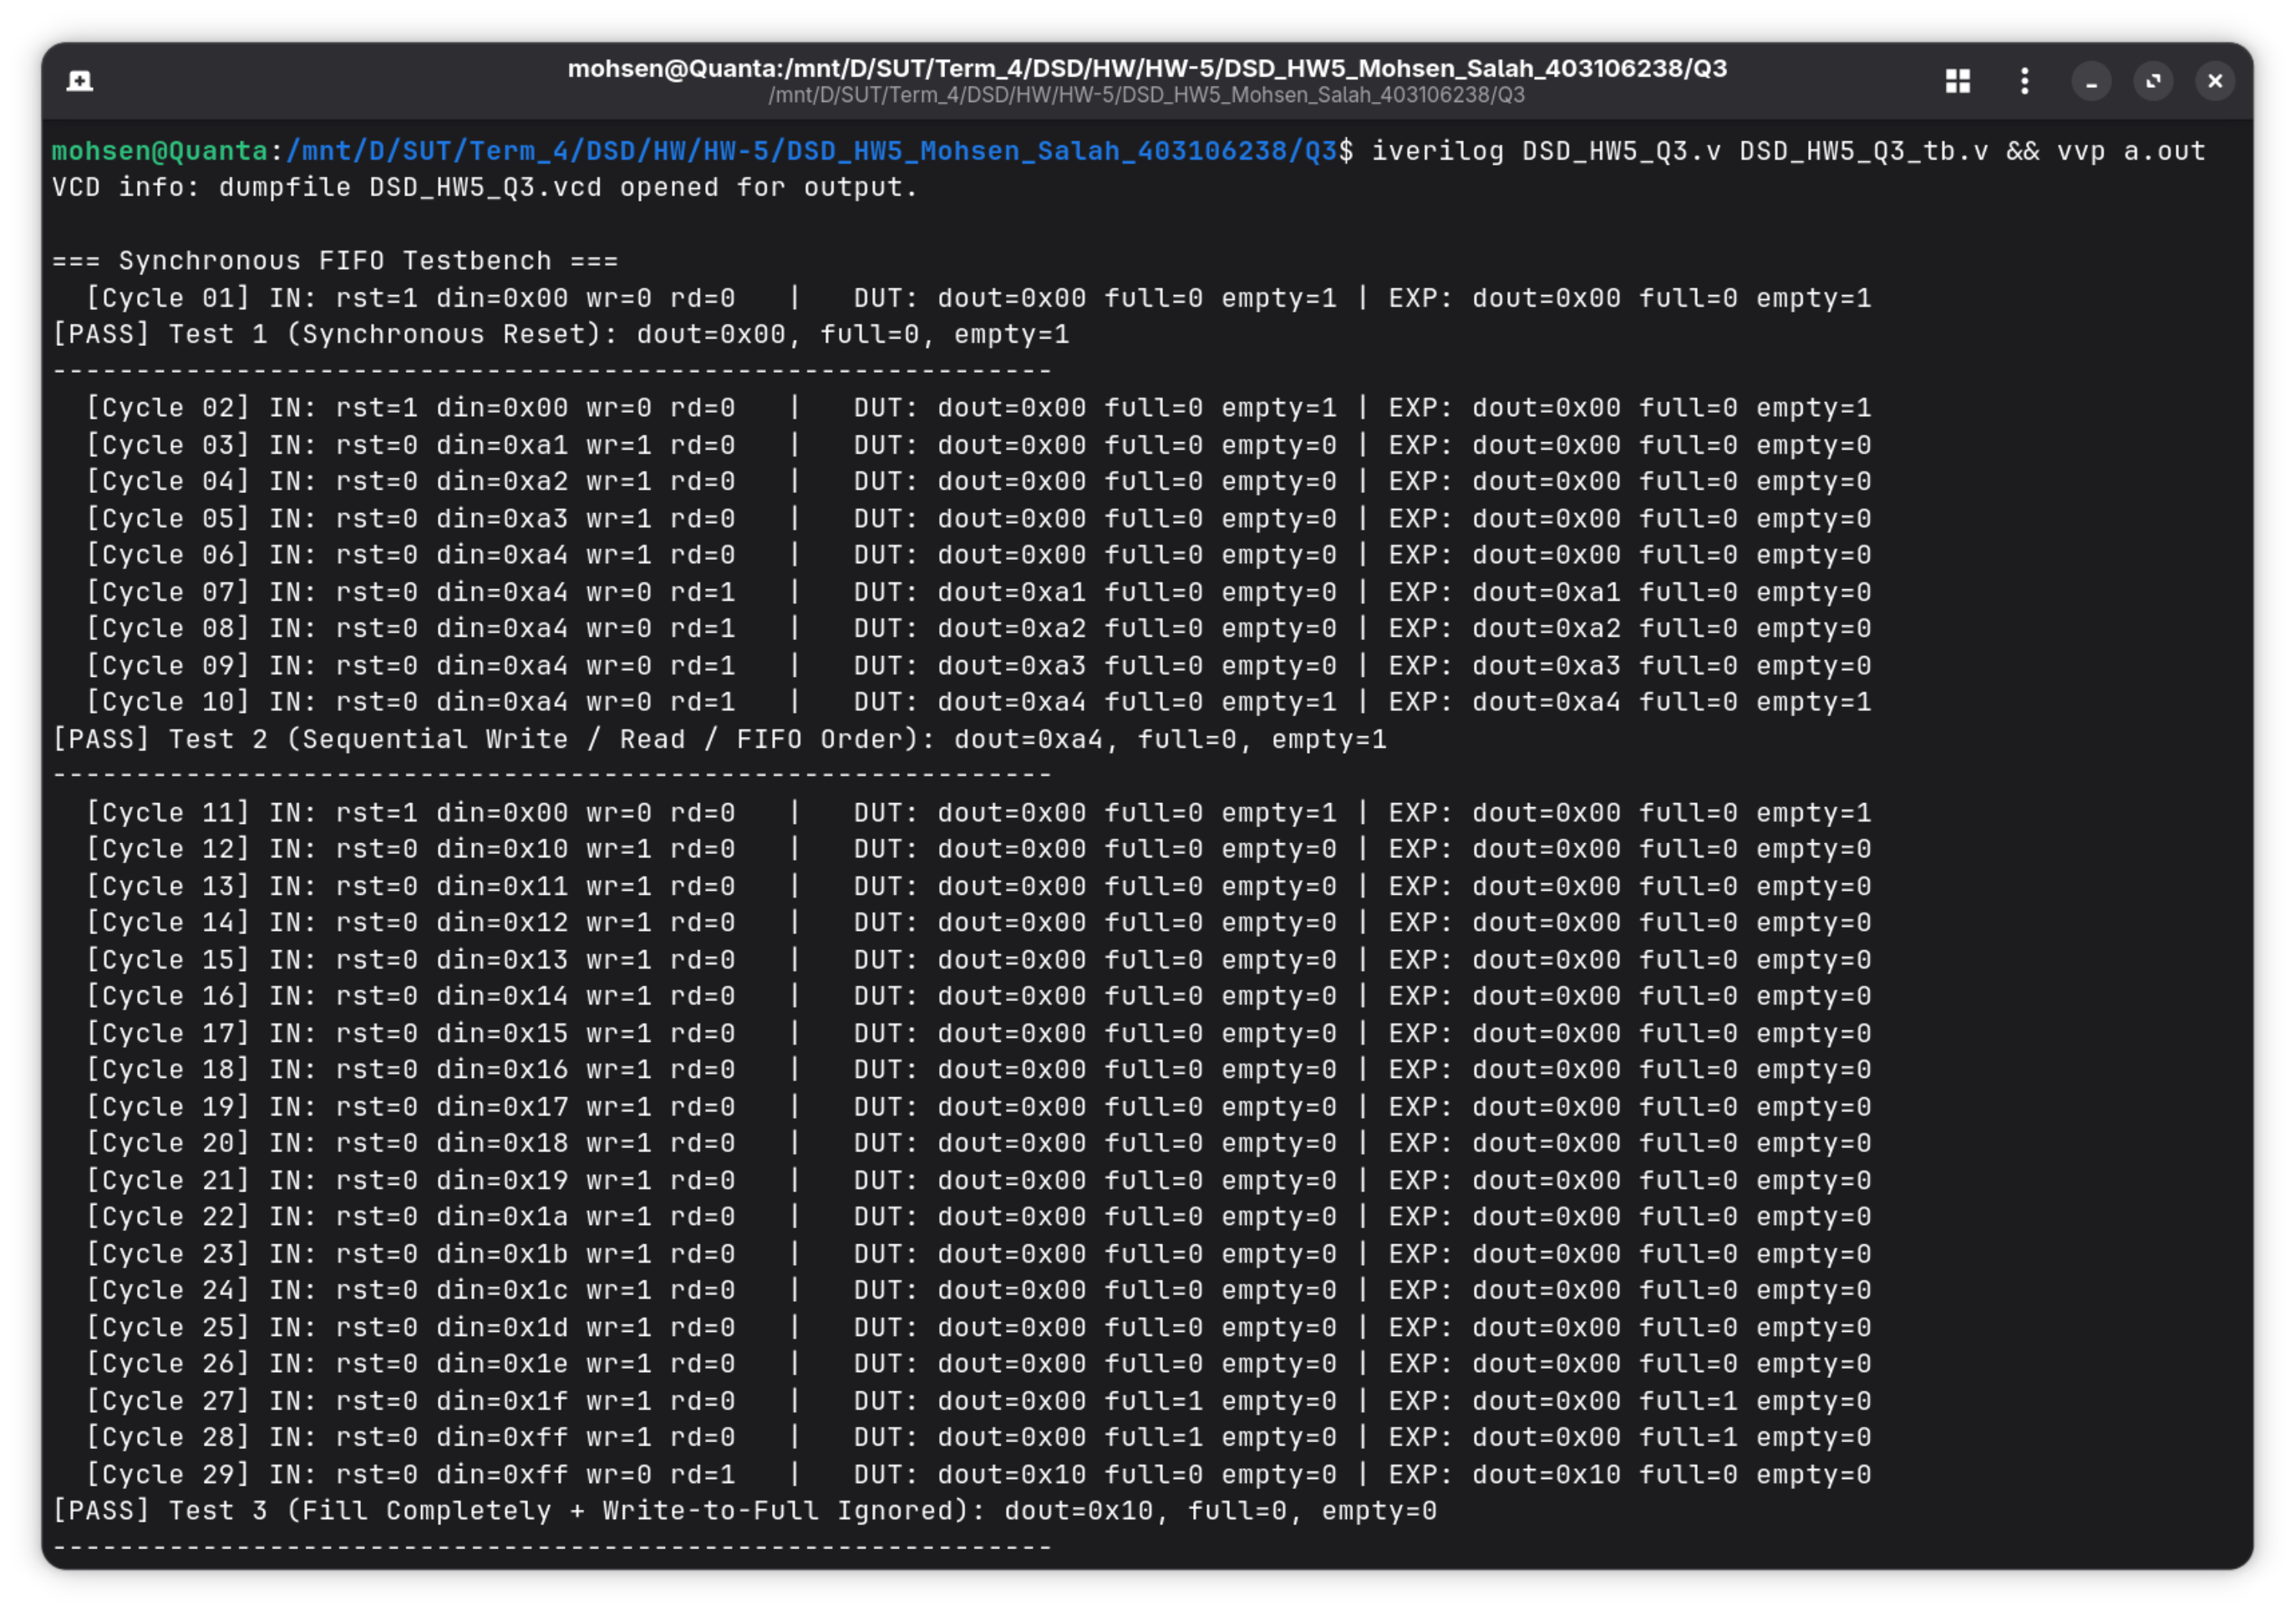
\includegraphics[width=0.9\textwidth]{assets/terminal_1.png}
    \caption{خروجی تست‌بنچ در ترمینال}
\end{figure}

\begin{figure}[H]
    \centering
    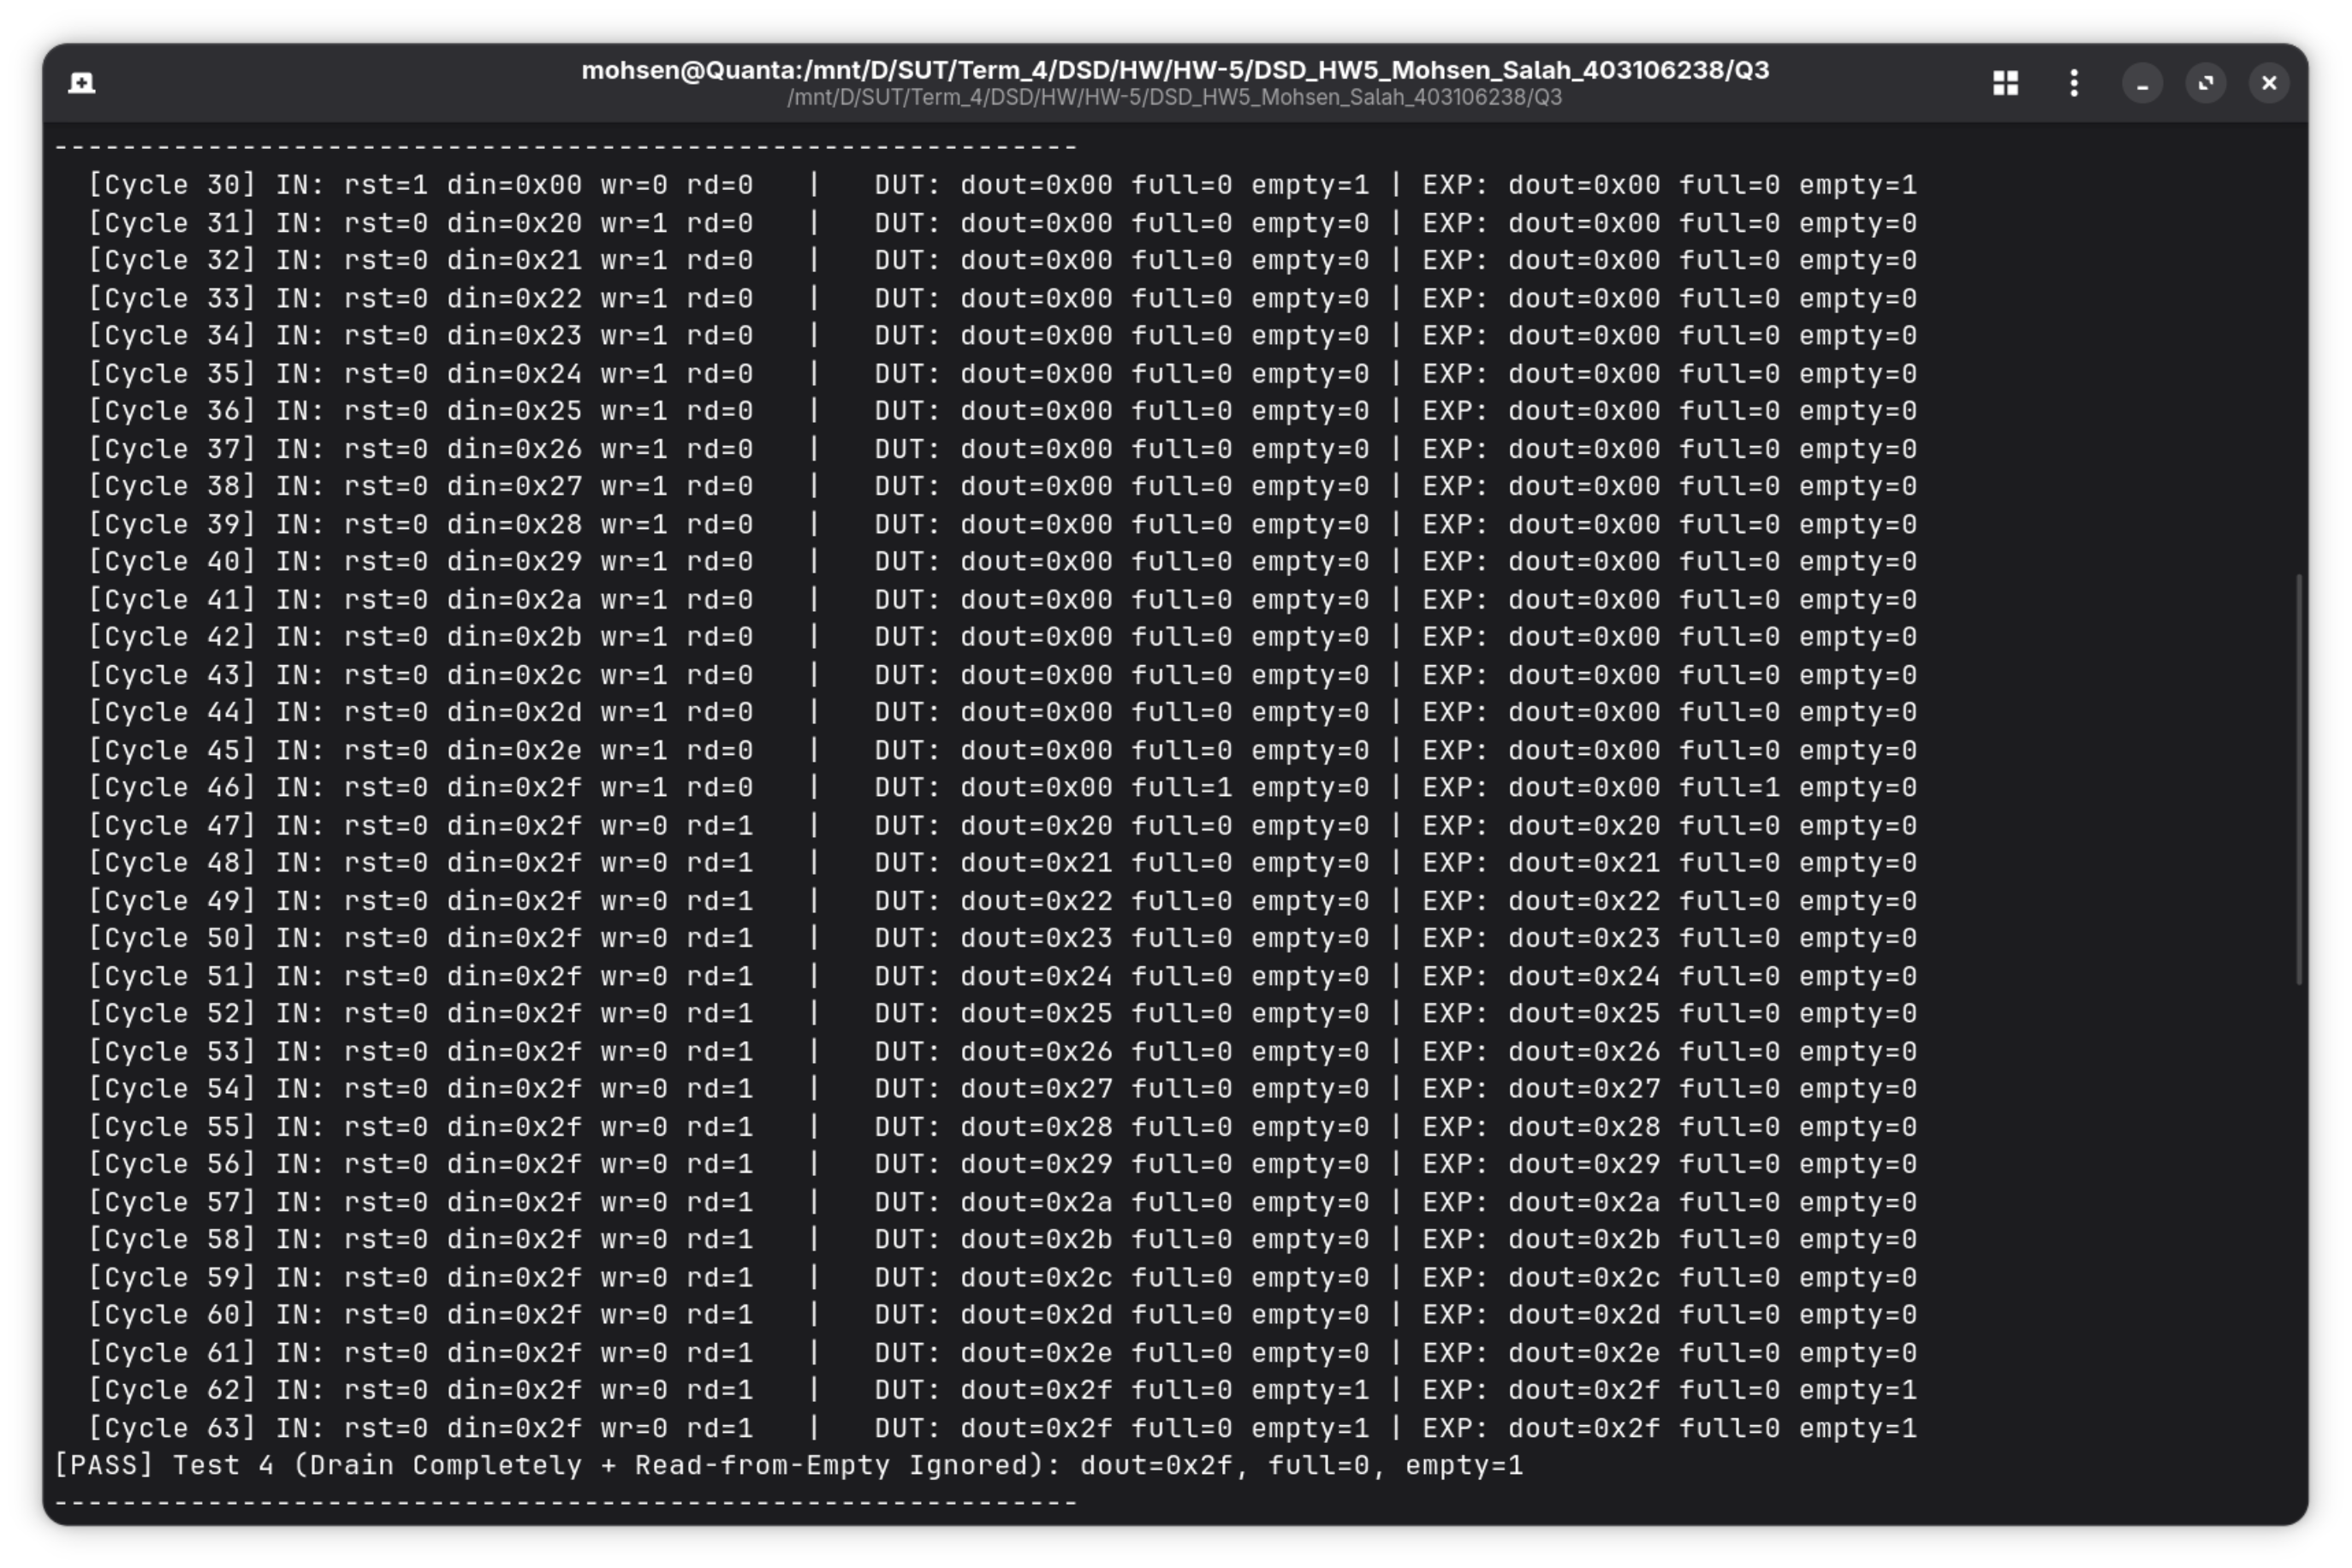
\includegraphics[width=0.9\textwidth]{assets/terminal_2.png}
    \caption{خروجی تست‌بنچ در ترمینال (ادامه)}
\end{figure}

\begin{figure}[H]
    \centering
    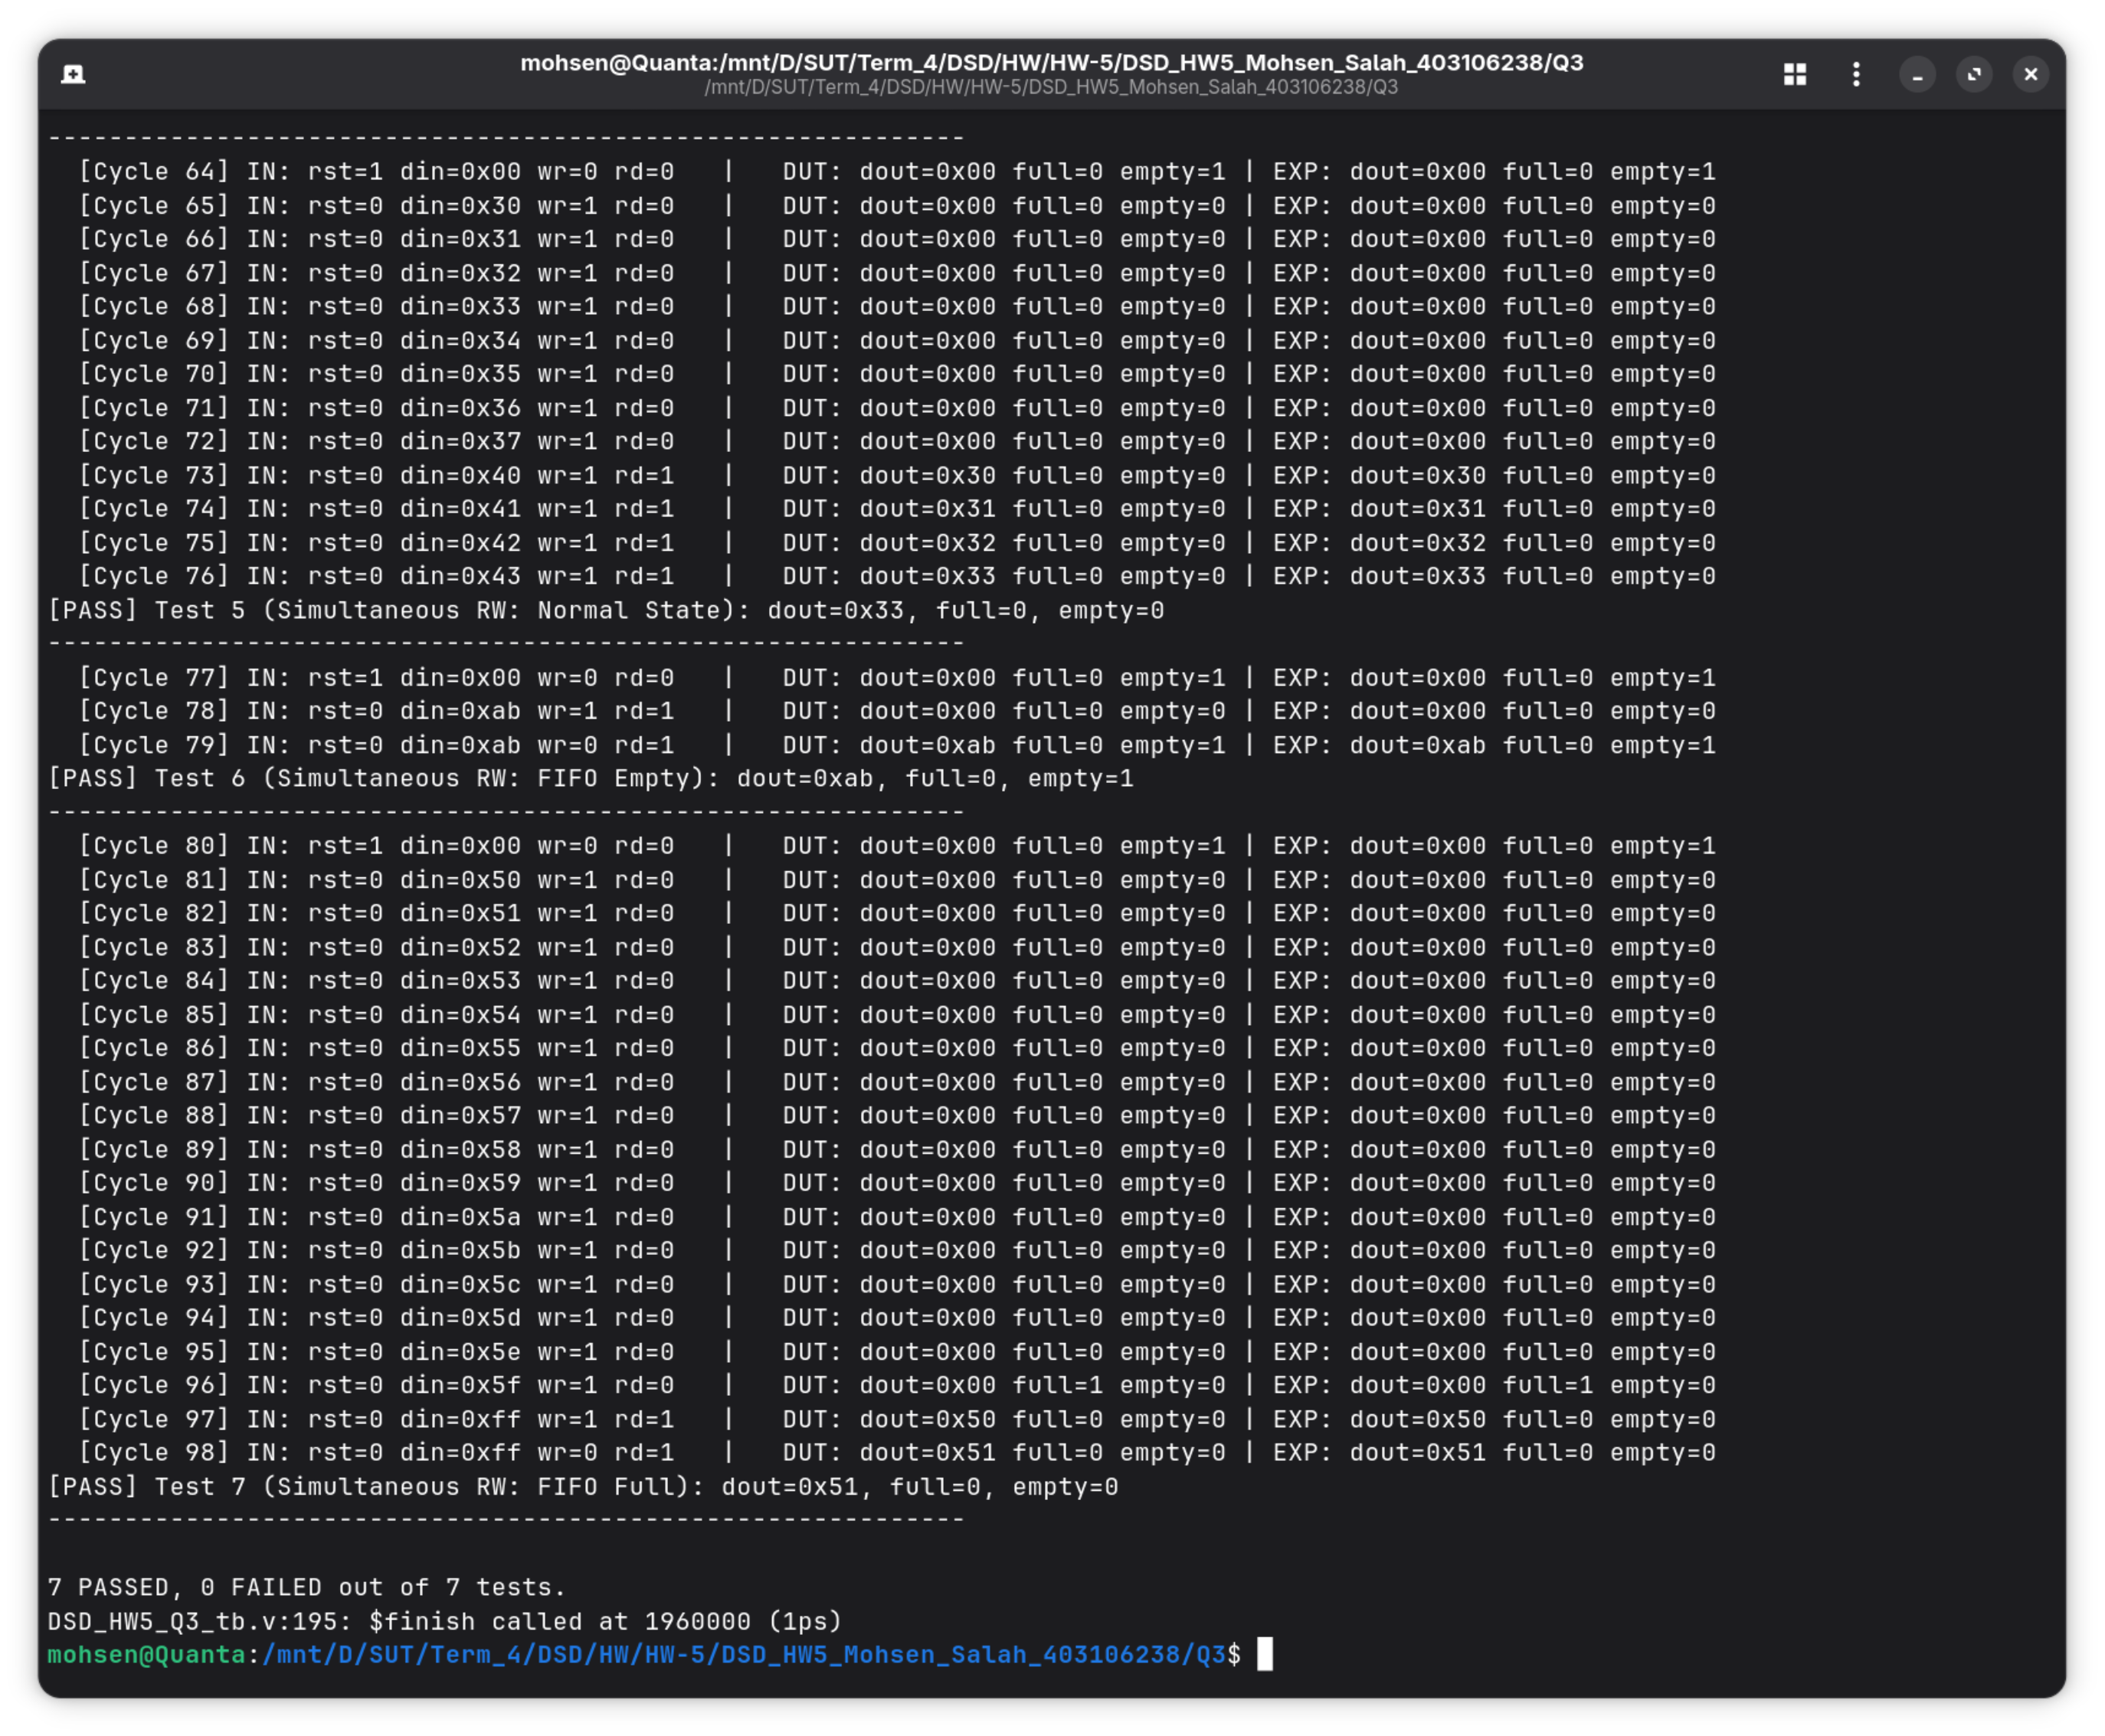
\includegraphics[width=0.9\textwidth]{assets/terminal_3.png}
    \caption{خروجی تست‌بنچ در ترمینال (ادامه)}
\end{figure}

همان طور که مشاهده می‌شود، تمامی ۷ تست‌کیس با موفقیت \lr{PASS} شده‌اند.

شکل موج سیگنال‌ها در \lr{GTKWave} نیز به این صورت می‌باشد:

\begin{figure}[H]
    \centering
    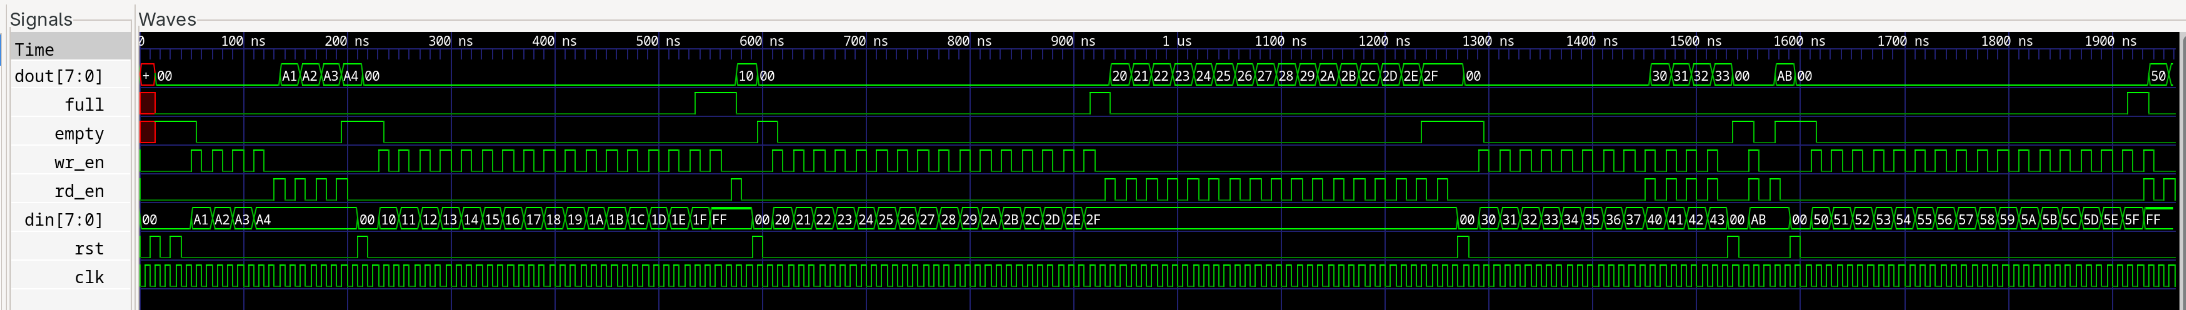
\includegraphics[width=1.0\textwidth]{assets/gtkwave.png}
    \caption{شکل موج سیگنال‌ها در \lr{GTKWave}}
\end{figure}

همان طور که مشاهده می‌شود، تغییرات اشاره‌گرها، سیگنال‌های \code{full} و \code{empty} و داده‌های خروجی مطابق با رفتار مورد انتظار مدار عمل می‌کنند.